\documentclass[a4paper,12pt,french]{book}
\usepackage[margin=2cm]{geometry}
\usepackage[thinfonts]{uglix2}
\begin{document}
\chapter*{\large Interaction entre l'homme et la machine sur le web\\[-1em]\fontsize{35pt}{42pt}\selectfont\titlefont JavaScript}

\double
{
\textsc{JavaScript} est un langage de programmation écrit en 1995 par Brendon Eich, alors qu'il travaillait chez Netscape Communication (entreprise pionnière dans le développement du web, qui a développé Netscape Navigator, un navigateur très populaire dans les années 90).\\
Ce langage permet d'interagir avec les éléments d'une page web et ainsi de dynamiser cette page.\\
Dans ce court chapitre nous verrons quelques exemples très simples d'utilisation de \textsc{JavaScript}.
}
{
	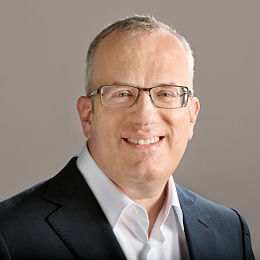
\includegraphics[width=4cm]{img/Brendan_Eich.jpg}
	\begin{center}
		Brendan Eich
	\end{center}
}
{4cm}

\begin{exercice}[]
	Dans \textsc{PyCharm}, ouvrir le dossier \tw{'pages avec JS'}.\\
	Pour chacun des 5 fichiers \tw{index} fournis, dans l'ordre :
	\begin{enumerate}[--]
		\item 	l'exécuter;
		\item 	lire le code  \textsc{HTML} (en utilisant \texttt{Ctrl+U} ou dans \textsc{PyCharm} ou \textsc{Notepad++});
		\item 	ouvrir le fichier \tw{.js}  (dans \textsc{PyCharm} ou \textsc{Notepad++}) correspondant et lire son code;
	\end{enumerate}
	Le but est de comprendre par soi-même comment \textsc{JavaScript} a été utilisé pour rendre la page dynamique.
\end{exercice}

\begin{exercice}[]
	\begin{enumerate}[\bfseries 1.]
		\item 	Chercher sur internet comment on crée une \textit{table} en \textsc{HTML}.
		\item 	Produire une page avec une table comportant 10 boutons affichant les chiffres de 0 à 9.
		\item 	En s'inspirant des pages de l'exercice précédent, afficher dynamiquement le contenu d'une variable \tw{somme} qui augmente au fur et à mesure qu'on appuie sur les boutons.
	\end{enumerate}
\end{exercice}

\begin{exercice}[ (facultatif)]
	Reprendre l'exercice précédent et le modifier pour produire une petite calculatrice.\\
	À chacun de décider de la complexité de la calculatrice : on peut s'arrêter à une simple machine à ajouter, on peut ajouter d'autres opérations...
\end{exercice}

\end{document}
	
